
% ===========================
\chapter{Umsetzung}
\label{umsetzung}
% ===========================

In diesem Kapitel wird die Umsetzung des Konzepts aus dem vorherigen Kapitel beschrieben. Zu Beginn werden die dafür notwendigen Fahrszenarien in Abschnitt \ref{umsetzung_definition} definiert. Danach wirda in den Abschnitten \ref{umsetzung_daten_synth} und \ref{umsetzung_daten_real} die Methodik für die Generierung von synthetische Trainingsdaten und reale Trainings- und Testdaten erläutert. Im Anschluss wird in Abschnitt \ref{umsetzung_training} die Architektur und die Experimente des Klassifikators für die Szenarienerkennung beschrieben.


% ===========================
\section{Definition der Fahrszenarien}
\label{umsetzung_definition}
% ===========================

In diesem Abschnitt werden Szenarien, wie in Abschnitt \ref{grundlagen_fahren_szenarien} beschrieben, als \textit{logische Szenarien} für das weitere Vorgehen in dieser Arbeit definiert. In Anlehnung an bestehende Arbeiten zu Erkennung von Fahrszenarien und auf Basis von Machbarkeitsabschätzungen für die Umsetzung werden in dieser Arbeit die Szenarien \textit{free cruising}, \textit{approaching} \textit{following}, \textit{catching up}, \textit{overtaking}, \textit{lane change left} und \textit{lane change right} auf der Autobahn betrachtet. Die Autobahn wurde ausgewählt, weil es weniger Parameter zu betrachten gibt als auf anderen Straßen wie beispielsweise in der Stadt. In der folgenden Tabelle \ref{tab_definition_szenarios} werden diese Szenarien auf \textit{funktionaler} und \textit{logischer Ebene} definiert.

Um die Darstellung in der Tabelle zu erleichtern werden folgende Abstände zwischen Ego-Fahrzeug und Fahrzeug 2 definiert. Dabei beschreibt $ego_v$ die Geschwindigkeit des Ego-Fahrzeugs in [m/s].

\begin{equation*}
\begin{split}
s_0 = ego_v * 3,6 \qquad \text{[m]} \\
s_1 = ego_v * 3,6 * \frac{2}{3} \qquad \text{[m]} \\
s_2 = ego_v * 3,6 * \frac{1}{2} \qquad \text{[m]} \\
s_3 = ego_v * 3,6 * \frac{1}{3} \qquad \text{[m]} \\
\end{split}
\end{equation*}

\small
\begin{longtable}[c]{p{2cm} p{5.5cm} p{6cm}}
\textbf{Szenario} & \textbf{Funktionale Definition} & \textbf{Logische Definition} \\
\hline
\endhead

\textbf{Alle} & 2-spurige Autobahn geradeaus oder in einer Kurve, Geschwindigkeitsbegrenzung ist größer als 80 km/h & Breite Fahrstreifen [2,3..3,5] m \newline Geschwindigkeitsbegrenzung [80..keine] km/h \\
\hline

\textbf{Alle} & Tageslicht, keine Wolken bis leicht bewölkt, kein Niederschlag, gute Sichtbedingungen & Tageszeit [Sonnenaufgang..Sonnenuntergang] \newline Bewölkung [leicht bewölkt..wolkenlos]\\
\hline \hline

\textbf{Free cruising} & Ego, andere Verkehrsteilnehmer \newline \underline{Interaktion:} Ego fährt frei auf linker oder rechter Fahrspur, andere Fahrzeuge sind weit entfernt und haben keinen Einfluss auf die Manöver des Ego & Geschwindigkeit Ego [60..200] km/h \newline Abstand zu anderen Verkehrsteilnehmern [$>s_0$] m \\
\hline

\textbf{Approaching} & Ego, andere Verkehrsteilnehmer \newline \underline{Interaktion:} Ego nähert sich auf linker oder rechter Fahrspur in mittlerem Abstand dem Fahrzeug 2 & Geschwindigkeit Ego abnehmend [60..200] km/h \newline Geschwindigkeit Ego < Geschwindigkeit Fahrzeug 2 \newline Abstand Ego zu Fahrzeug 2 [$s_2$..$s_0$] m \\
\hline

\textbf{Following} & Ego, andere Verkehrsteilnehmer \newline \underline{Interaktion:} Ego fährt auf linker oder rechter Fahrspur in sicherem Abstand hinter Fahrzeug 2 & Geschwindigkeit Ego [60..200] km/h \newline Geschwindigkeitsdifferenz zwischen Ego und Fahrzeug 2 < Geschwindigkeit Ego $*0,05$ km/h \newline Abstand Ego zu Fahrzeug 2 [$s_3$..$s_1$] m \newline Ego befindet sich auf gleicher Fahrspur hinter Fahrzeug 2 \\
\hline

\textbf{Catching up} & Ego, andere Verkehrsteilnehmer \newline \underline{Interaktion:} Ego fährt auf linker Fahrspur und verringert den vertikalen Abstand zu Fahrzeug 2 auf der rechten Fahrspur (auf-/überholen) & Geschwindigkeit Ego [60..200] km/h \newline Geschwindigkeit Fahrzeug 2 < Geschwindigkeit Ego \newline Vertikaler Abstand Ego zu Fahrzeug 2 [0..$s_0$] m \newline Ego fährt auf linker Fahrspur hinter Fahrzeug 2 das auf rechter Fahrspur fährt \\
\hline

\textbf{Overtaking} & & \\
\hline

\textbf{Lane change left} & Ego, andere Verkehrsteilnehmer sind optional \newline \underline{Interaktion:} Ego fährt auf rechter Fahrspur und wechselt auf linke Fahrspur & Geschwindigkeit Ego [60..200] km/h \newline Ego befindet sich auf rechter Fahrspur und wechselt auf linke Fahrspur \\
\hline

\textbf{Lane change right} & Ego, andere Verkehrsteilnehmer sind optional \newline \underline{Interaktion:} Ego fährt auf linker Fahrspur und wechselt auf rechte Fahrspur & Geschwindigkeit Ego [60..200] km/h \newline Ego befindet sich auf linker Fahrspur und wechselt auf rechte Fahrspur \\
\hline

\caption{Definition der Szenarien \textit{free cruising}, \textit{approaching}, \textit{following}, \textit{catching up}, \textit{overtaking}, \textit{lane change left} und \textit{lane change right}}
\label{tab_definition_szenarios}
\end{longtable}
\normalsize

% ===========================
\section{Generierung synthetischer Trainingsdaten}
\label{umsetzung_daten_synth}
% ===========================

Auf Basis der Definitionen aus dem vorherigen Abschnitt \ref{umsetzung_definition} werden in diesem Abschnitt die benötigten Signal- und Bilddaten simuliert und entsprechend gelabelt. Dafür werden in Abschnitt \ref{umsetzung_daten_synth_simulation} die Signaldaten, die für die eindeutige Klassifizierung der Szenarien benötigt werden, simuliert. In Abschnitt \ref{umsetzung_daten_synth_labeling} werden diese Signaldaten verwendet um die parallel simulierten Bilddaten entsprechend zu labeln.
 
% ===========================
\subsection{Simulation mit CarMaker}
\label{umsetzung_daten_synth_simulation}
% ===========================

Für die Simulation der Signal- und Bilddaten wird die kommerzielle Software CarMaker von IPG Automotive \cite{ipg2018carmaker} verwendet. Diese Simulationssoftware wird für den virtuellen Fahrversuch und \ac{HiL}-Tests eingesetzt um Komponenten in unterschiedlichen Szenarien zu testen. In dieser Arbeit wird CarMaker verwendet, um die Szenarien \textit{free cruising}, \textit{approaching}, \textit{following}, \textit{catching up}, \textit{overtaking}, \textit{lane change left} und \textit{lane change right} zu simulieren.

Für die Aufnahme der benötigten Bilddaten wird im simulierten Fahrzeug ein entsprechender Kamerasensor konfiguriert. Die Konfiguration des Sensors orientiert sich an der Konfiguration von realen Frontview-Kameras im Fahrzeug nach Punke \cite{punke2015kamera}. So ist der Kamerasensor an der Stelle des Rückfahrspiegels platziert und hat eine Auflösung von 640 x 480 Pixeln und ein Sichtfeld von 20°.

Die benötigten Signaldaten für das Labeln werden von den Definitionen aus Abschnitt \ref{umsetzung_definition} abgeleitet. Für die eindeutige Identifikation der logischen Szenarien werden die folgenden Werte benötigt: Geschwindigkeit des Ego-Fahrzeugs, Abstand und Geschwindigkeitsdifferenz des Ego-Fahrzeugs zu allen anderen Fahrzeugen, aktuelle Fahrspur des Ego-Fahrzeugs und allen anderen Fahrzeugen und die relative Position des Ego-Fahrzeugs, i.e. ob sich das Ego-Fahrzeug vor oder hinter einem anderen Fahrzeug befindet. Um den Abstand und die Geschwindigkeitsdifferenz des Ego-Fahrzeugs zu allen anderen Fahrzeugen aufzuzeichnen, wird ein Objektsensor im Ego-Fahrzeug konfiguriert. Mit diesem Sensor können im konfigurierten Radius alle Fahrzeuge und ihr Abstand und ihre relative Geschwindigkeit zum Ego-Fahrzeug erfasst und über die \textit{OutputQuantities} in CarMaker aufgezeichnet werden. Die Geschwindigkeit des Ego-Fahrzeugs und die Fahrspur-ID und Position aller Fahrzeuge können direkt, ohne zusätzlichen Sensor, über die \textit{OutputQuantities} aufgezeichnet werden. Die jeweiligen Variablen in CarMaker sind in der Tabelle \ref{tab_output_quantities} zusammengefasst.

\begin{table}[h]
\small
\centering
\def\arraystretch{1.4}
\begin{tabular}{p{6.2cm} p{7.5cm}}
\textbf{Variable in CarMaker} & \textbf{Beschreibung} \\
\hline

Car.v & Geschwindigkeit des Ego-Fahrzeugs in [m/s] \\
Car.Road.sRoad & Position des Ego-Fahrzeugs auf der Strecke in [m] \\
Car.Road.Lane.Act.LaneId & Fahrspur-ID des Ego-Fahrzeugs \\
\hline
Sensor.Object.OB01.TX.NearPnt.dv\_p & Geschwindigkeitsdifferenz zwischen Fahrzeug TX und dem Ego-Fahrzeug in [m/s] \\
Sensor.Object.OB01.TX.NearPnt.ds\_p & Abstand zwischen Fahrzeug TX und dem Ego-Fahrzeug in [m] \\
\hline
Traffic.TX.sRoad & Position des Fahrzeugs TX auf der Strecke in [m] \\
Traffic.TX.Lane.Act.LaneId & Fahrspur-ID des Fahrzeugs TX \\
\hline

\end{tabular}
\caption{Aufgezeichnete Signaldaten in CarMaker}
\label{tab_output_quantities}
\end{table}

Für die Simulation werden zwei Strecken der Länge 6.000m und 10.000m mit dem \textit{CarMaker - Scenario Editor} erstellt. Bei beiden Strecken handelt es sich um eine 4-spurige Autobahn mit zwei Fahrspuren in jede Richtung. Die Fahrtrichtungen sind in der Mitte von einer Leitplanke getrennt und am Rand der Fahrbahn sind jeweils Standstreifen vorhanden. Abschnittsweise stehen neben der Fahrbahn auch einige Bäume, was in Abbildung \ref{fig_cm_road_strecke} mit grünen Streifen gekennzeichnet ist. Abbildung \ref{fig_cm_road_bild} zeigt die Konfiguration der simulierten Straße.

\begin{figure}[h]
\centering
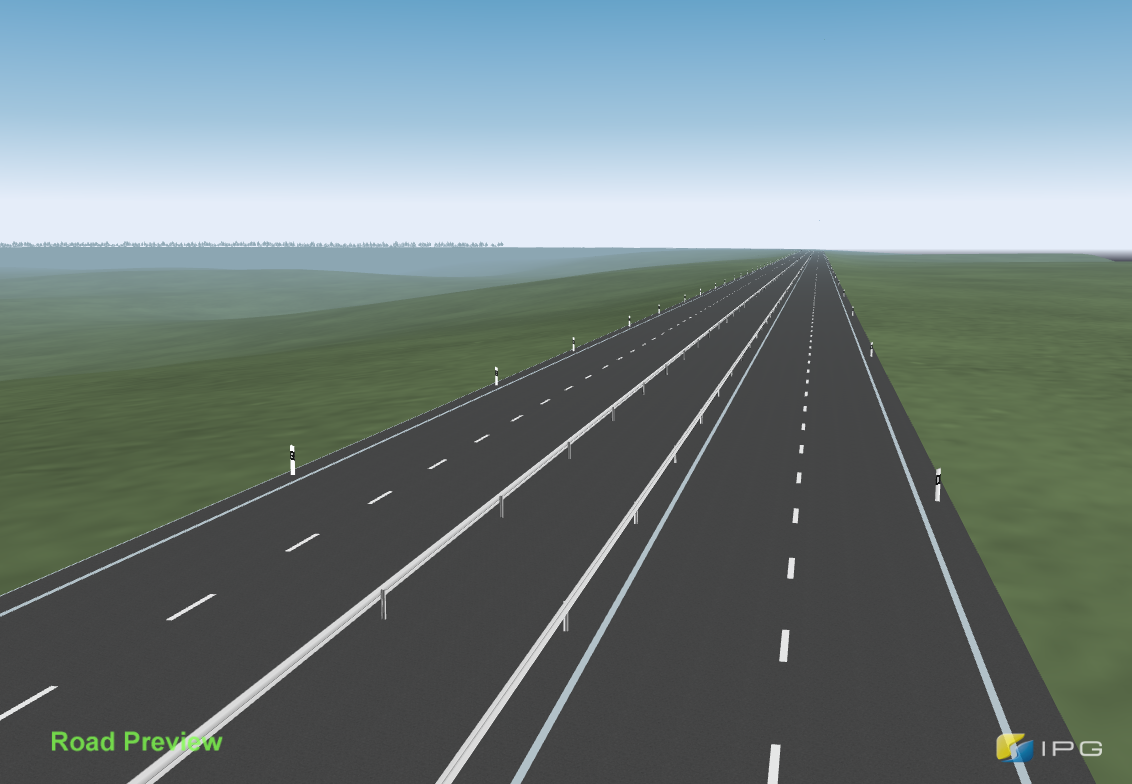
\includegraphics[scale=0.4]{cm_road_bild.png}
\caption{Konfiguration der simulierten Straße \cite{ipg2018carmaker}}
\label{fig_cm_road_bild}
\end{figure}

Auf beiden Strecken wird autonomer, stochastisch verteilter Verkehr erzeugt, was CarMaker mit einer gesonderten Funktion unterstützt. Der Verkehr wird in einer niedrigen Dichte (10\%) und einem 80\%-igen Anteil Autos erzeugt, andere Fahrzeuge sind Motorräder, Lastkraftwagen und Busse. In CarMaker ist eine Vielzahl an unterschiedlichen Fahrzeugen verfügbar, was wichtig ist um möglichst viele unterschiedliche Szenarien zu generieren. Mit dieser Konfiguration werden auf der 10.000m-Strecke 131 Fahrzeuge und auf der 6.000m-Strecke 89 Fahrzeuge generiert.

\begin{figure}[h]
\centering
\begin{tabular}{c}
\subfloat[Strecke 1]{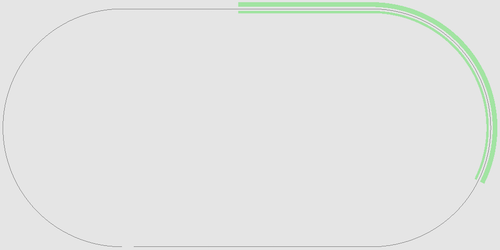
\includegraphics[scale=0.8]{cm_road_1.png}} \\
\subfloat[Strecke 2]{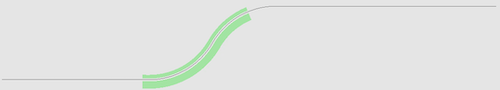
\includegraphics[scale=0.8]{cm_road_2.png}}
\end{tabular}
\caption{Schema der simulierten Strecken 1 und 2 \cite{ipg2018carmaker}}
\label{fig_cm_road_strecke}
\end{figure}

Die Simulation und Generierung von Bild- und Signaldaten wird mit dem \textit{CarMaker - Test Manager} durchgeführt. Mit diesem Modul lassen sich Fahrten mit unterschiedlichen Konfigurationen simulieren. In dieser Arbeit werden die Variablen \textit{Geschwindigkeit}, \textit{Mindestabstand zu vorausfahrendem Fahrzeug}, \textit{Minimale Geschwindigkeitsdifferenz beim Überholen} und \textit{Aggressivität beim Überholen} auf beiden oben beschriebenen Strecken variiert. Die Werte der Variablen, die simuliert werden, sind in Tabelle \ref{tab_tm_variablen} aufgelistet und sind aus der Sicht des Ego-Fahrzeugs.

\begin{table}[h]
\small
\centering
\def\arraystretch{1.4}
\begin{tabular}{p{8cm} p{0.7cm} p{0.7cm} p{0.7cm} p{0.7cm} p{0.7cm}}
\textbf{Variable} & \textbf{Werte} & & & & \\
\hline
Geschwindigkeit in [km/h] & 100 & 120 & 140 & 160 & 180 \\
Mindestabstand zu vorausfahrendem Fahrzeug in [s] & 1,0 & 1,5 & 2,0 & & \\
Minimale Geschwindigkeitsdifferenz beim Überholen in [km/h] & 5 & 15 & 25 & & \\
Aggressivität beim Überholen & 0,2 & 0,6 & 1,0 & & \\
\hline
\end{tabular}
\caption{Variablen und Werte die in der Simulation verwendet werden}
\label{tab_tm_variablen}
\end{table}

Die ersten drei Variablen sind selbsterklärend und werden hier nicht weiter erläutert. Die Variable \textit{Aggressivität beim Überholen} (in CarMaker \textit{Overtaking Rate} ist eine Zahl zwischen 0 und 1. Dabei markiert die 0 ein Fahrstil, bei dem sich der Fahrer sehr risikoavers beim Überholen verhält, i.e. Überholen nur in sehr sicheren Situationen. Je größer die Zahl wird, desto aggressiver wird der Überholvorgang und dementsprechend sinkt die Risikoaversion beim Überholen und der Fahrer überholt auch bei kritischen oder schlecht einsehbaren Situationen.

Mit diesen vier Variablen mit jeweils drei bzw. fünf Werten ergeben sich 135 verschiedene Kombinationsmöglichkeiten. Somit werden auf beiden Strecken in Summe 270 Fahrten mit 2.160 km simuliert. Signal- und Bilddaten werden mit einer Frequenz von 5 Hz aufgezeichnet, was in 326.108 aufgezeichneten Szenen (Bilder und Signaldaten) resultiert. Diese Szenen werden im folgenden Abschnitt \ref{umsetzung_daten_synth_labeling} gelabelt.


% ===========================
\subsection{Daten Labeling}
\label{umsetzung_daten_synth_labeling}
% ===========================

Für das Labeln der Szenarien wird jede Szene auf Basis der Definition aus Abschnitt \ref{umsetzung_definition} mithilfe der Signaldaten klassifiziert. Die logischen Bedingungen für jedes Szenario sind dafür in Tabelle \ref{tab_szenarien_labeling} aufgelistet. Auf Basis der CarMaker-Variablen aus Tabelle \ref{tab_tm_variablen} werden folgende zusätzliche Variablen definiert, um nachfolgende Bedingungen übersichtlicher darzustellen. Dabei beschreibt $v2$ jeweils das Fahrzeug, auf Basis dessen das jeweilige Szenario klassifiziert wird.

\begin{equation*}
\begin{split}
ego_v = \text{Car.v} \qquad \text{[m/s]} \\
ego_{sRoad} = \text{Car.Road.sRoad} \qquad \text{[m]} \\
ego_{laneID} = \text{Car.Road.Lane.Act.LanId} \qquad \text{[1, 2]} \\
v2_{dv} = \text{Sensor.Object.OB01.TX.NearPnt.dv\_p} \qquad \text{[m/s]} \\
v2_{ds} = \text{Sensor.Object.OB01.TX.NearPnt.dv\_p} \qquad \text{[m]} \\
v2_{sRoad} = \text{Traffic.TX.sRoad} \qquad \text{[m]} \\
v2_{laneID} = \text{Traffic.TX.Lane.Act.LaneId} \qquad \text{[1, 2]} \\
\end{split}
\end{equation*}

\small
\begin{longtable}[c]{p{3cm} p{8.5cm}}
\textbf{Szenario} & \textbf{Bedingungen} \\
\hline
\endhead

\textbf{Free cruising} & $ego_v > 17$ \newline $s_0 < v2_{ds}$ \\
\hline
\textbf{Approaching} & $s_2 < v2_{ds} < s_0$ \newline $ego_{sRoad} < v2_{sRoad}$ \newline $ego_{laneID} == v2_{laneID}$ \newline $ego_v < \text{ Durchschnitt von } ego_v \text{ der letzten 3 Sekunden} $ \\
\hline
\textbf{Following} & $v2_{dv} < ego_v * 0,05$ \newline $s_3 < s_1$ \newline $ego_{sRoad} < v2_{sRoad}$ \newline $ego_{laneID} == v2_{laneID}$ \\
\hline
\textbf{Catching up} & $v2_{dv} < 0$ \newline $0 <= v2_{ds} < s_0$ \newline $ego_{sRoad} <= v2_{sRoad}$ \newline $ego_{laneID} == v2_{laneID} - 1$ \\
\hline
\textbf{Overtaking} & $0 <= v2_{ds} < s_0$ \newline $v2_{sRoad} < ego_{sRoad}$ \newline $ego_{laneID} == v2_{laneID} - 1$ \\
\hline
\textbf{Lane change left} & $ego_{laneID}^{before} == ego_{laneID}^{after} + 1$ \newline Als Spurwechsel wird ein Intervall von 4 Sekunden betrachtet in dessen Mitte die Variable ihren Wert wechseln muss\\
\hline
\textbf{Lane change right} & $ego_{laneID}^{before} == ego_{laneID}^{after} - 1$ \newline Als Spurwechsel wird ein Intervall von 4 Sekunden betrachtet in dessen Mitte die Variable ihren Wert wechseln muss \\

\hline
\caption{Bedingungen der Szenarien \textit{free cruising}, \textit{approaching}, \textit{following}, \textit{catching up}, \textit{overtaking}, \textit{lane change left} und \textit{lane change right}}
\label{tab_szenarien_labeling}
\end{longtable}
\normalsize

Im Anschluss an die Klassifizierung einzelner Zeitpunkte werden diese zu Szenarien zusammengefasst, wenn mindestens 15 Zeitpunkte (3 Sekunden) in Folge mit dem gleichen Label klassifiziert wurden. Drei Sekunden wird den folgenden zwei Gründen als Länge für Szenarien in dieser Arbeit gewählt. Erstens orientiert sich diese Zeitspanne an den vorherigen Arbeiten zur Szenarienerkennung. Zweitens haben die zwei Szenarien \textit{lane change left} und \textit{lane change right} jeweils eine natürliche Länge von 3-4 Sekunden. Alle anderen Szenarien können länger sein, lassen sich aber in Blöcke von jeweils 3 Sekunden einteilen. Insgesamt werden 326.108 Zeitpunkte und 23.972 Szenarien klassifiziert. Die Anzahl der simulierten Szenarien nach Klasse ist in der Tabelle \ref{tab_verteilung_szenarien} dargestellt.

\begin{table}[h]
\small
\centering
\def\arraystretch{1.4}
\begin{tabular}{l c}

\textbf{Szenario} & \textbf{Anzahl} \\
\hline
Free cruising & 2.545 \\
Approaching & 3.512 \\
Following & 3.601 \\
Catching up & 5.563 \\
Overtaking & 5.149 \\
Lane change left & 957 \\
Lane change right & 975 \\
Unknown & 1.670 \\
\hline
Summe & 23.972 \\
\hline

\end{tabular}
\caption{Anzahl der simulierten Szenarien nach Klasse}
\label{tab_verteilung_szenarien}
\end{table}

Es sind auch einige Szenarien als \textit{unknown} klassifiziert, da zwischen den definierten Szenarien andere Situationen auftreten können oder nicht die Mindestanzahl der konsekutiven Szenen erreicht wird. Zu manchen Zeitpunkten werden mehr als eine einzelne Szene klassifiziert. Beispielsweise kann sich das Ego-Fahrzeug gleichzeitig in der Szene \textit{catching up} und \textit{overtaking} befinden, wenn es auf der linken Fahrspur fährt und sich in vertikalem Abstand ein anderes Fahrzeug jeweils vor und hinter dem Ego-Fahrzeug befindet. Abbildung \ref{fig_beispiel_szenario_lcl} zeigt ein Beispiel des Szenarios \textit{lane change left} mit allen zugehörigen 15 Bildern.

\begin{figure}[h]
\centering
\begin{tabular}{c c c c c}
\subfloat[]{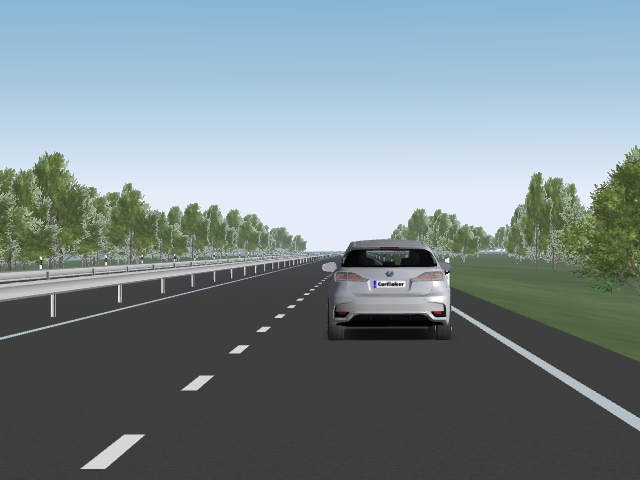
\includegraphics[scale=0.1]{lcl_sim/lcl0.jpg}} &
\subfloat[]{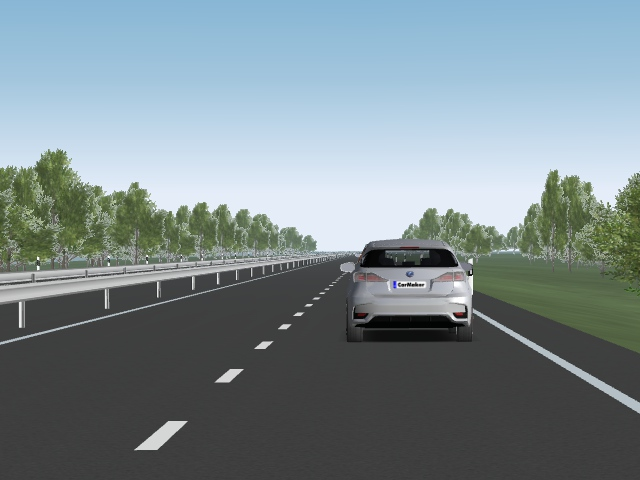
\includegraphics[scale=0.1]{lcl_sim/lcl1.jpg}} &
\subfloat[]{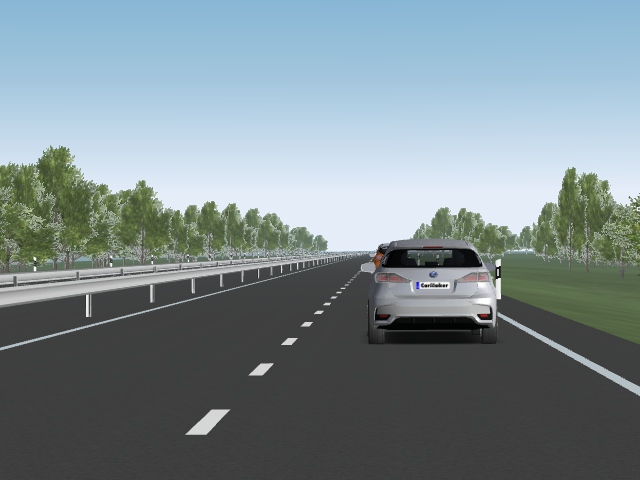
\includegraphics[scale=0.1]{lcl_sim/lcl2.jpg}} &
\subfloat[]{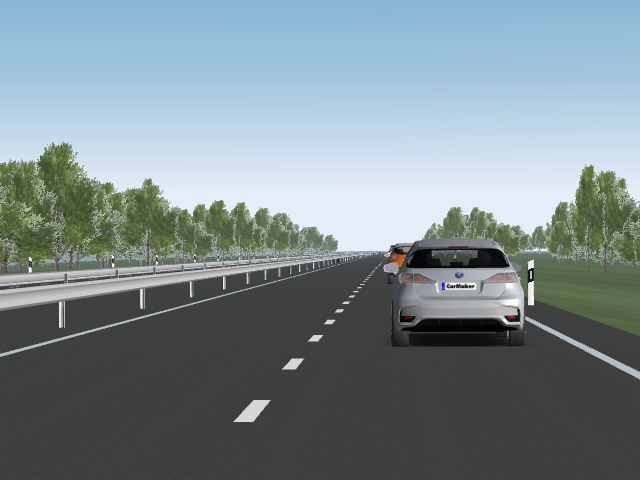
\includegraphics[scale=0.1]{lcl_sim/lcl3.jpg}} &
\subfloat[]{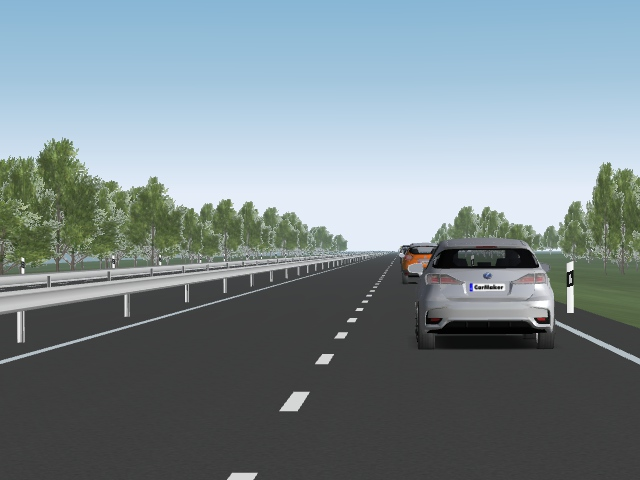
\includegraphics[scale=0.1]{lcl_sim/lcl4.jpg}} \\
\subfloat[]{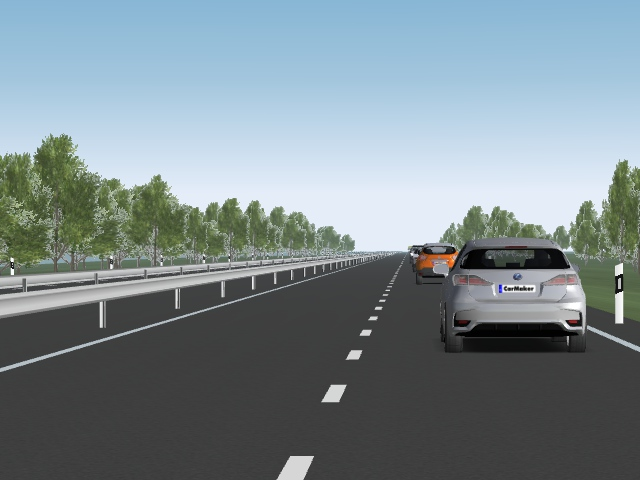
\includegraphics[scale=0.1]{lcl_sim/lcl5.jpg}} &
\subfloat[]{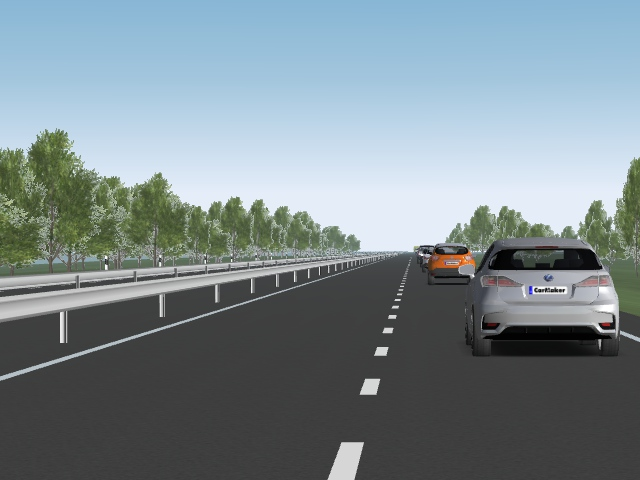
\includegraphics[scale=0.1]{lcl_sim/lcl6.jpg}} &
\subfloat[]{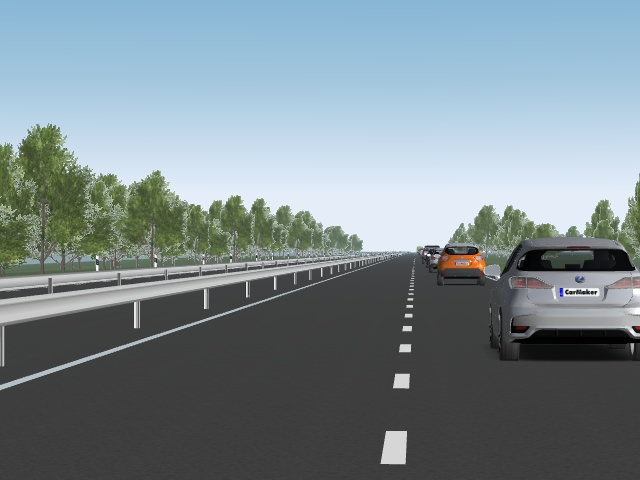
\includegraphics[scale=0.1]{lcl_sim/lcl7.jpg}} &
\subfloat[]{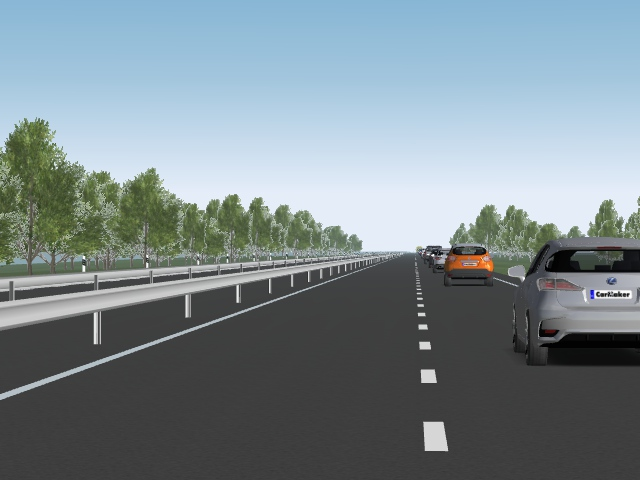
\includegraphics[scale=0.1]{lcl_sim/lcl8.jpg}} &
\subfloat[]{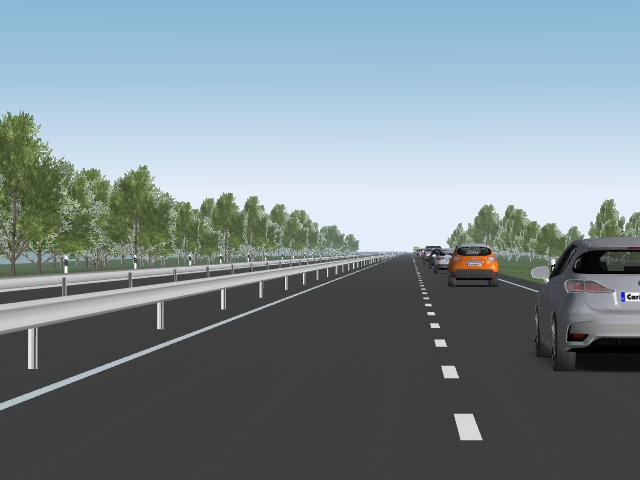
\includegraphics[scale=0.1]{lcl_sim/lcl9.jpg}} \\
\subfloat[]{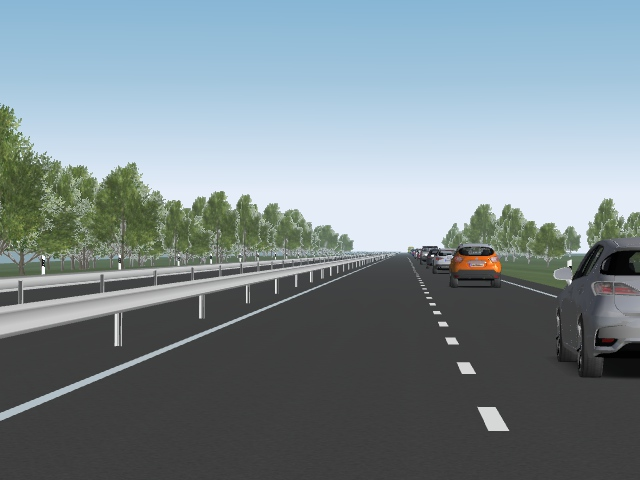
\includegraphics[scale=0.1]{lcl_sim/lcl10.jpg}} &
\subfloat[]{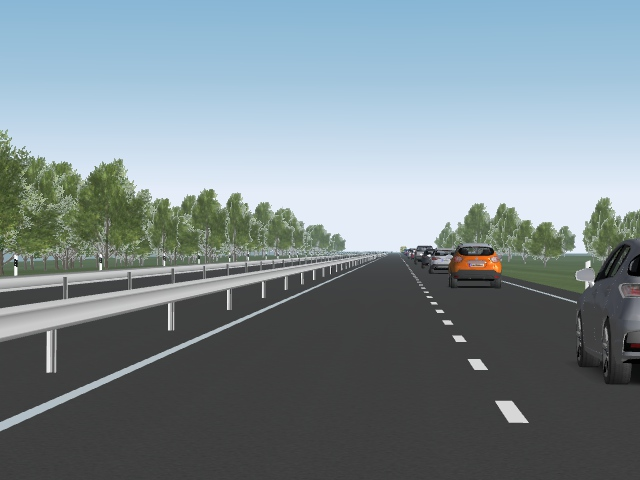
\includegraphics[scale=0.1]{lcl_sim/lcl11.jpg}} &
\subfloat[]{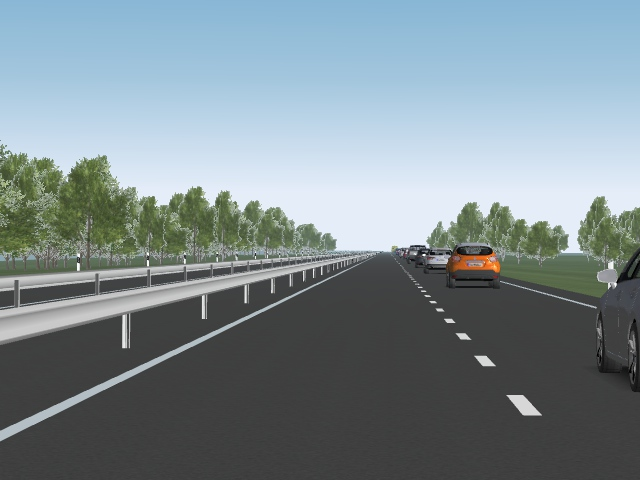
\includegraphics[scale=0.1]{lcl_sim/lcl12.jpg}} &
\subfloat[]{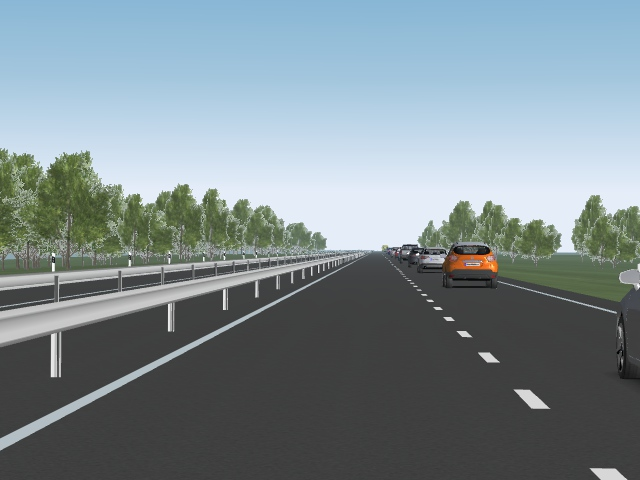
\includegraphics[scale=0.1]{lcl_sim/lcl13.jpg}} &
\subfloat[]{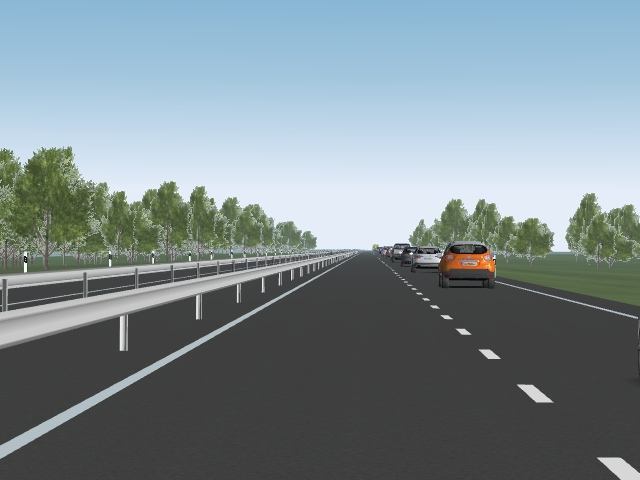
\includegraphics[scale=0.1]{lcl_sim/lcl14.jpg}} \\
\end{tabular}
\caption{Beispiel eines simulierten Szenarios der Klasse \textit{lane change left} \cite{ipg2018carmaker}}
\label{fig_beispiel_szenario_lcl}
\end{figure}


% ===========================
\section{Generierung realer Trainings- und Testdaten}
\label{umsetzung_daten_real}
% ===========================

Für den Proof-of-Concept dieser Arbeit, die Erkennung von realen Fahrszenarien, werden neben den synthetischen Trainingsdaten auch reale Daten für das Training und die anschließenden Tests benötigt. Dafür werden im ersten Schritt bestehen Datensätze nach ihrer Nutzbarkeit untersucht.

Die bekanntesten Datensätze sind KITTI \cite{geiger2013vision}, BDD100K \cite{yu2018bdd100k}, Cityscapes \cite{cordts2016cityscapes} und Oxford RobotCar \cite{maddern20171}. Der Cityscapes und Oxford RobotCar Datensatz umfasst lediglich Bilder von Szenen in Städten und ist daher nicht nutzbar für diese Arbeit. Die Datensätze KITTI und BDD100K umfassen auch Videos von Autobahnfahrten, allerdings liegt der Fokus auf Objekterkennung in einzelnen Bildern oder semantischer Segmentation. Und es gibt jeweils nur sehr begrenzt Videos, die auf einer 2-spurigen Autobahn aufgenommen wurden. Daher können diese Datensätze in dieser Arbeit nicht verwendet werden.

Als Alternative werden die Aufnahmen von zwei Fahrten auf der Autobahn und Bundesstraße verwendet. Die Strecken sind in der Abbildung \ref{fig_strecken_real} abgebildet. 

\begin{figure}[h]
\centering
\begin{tabular}{c c}
\subfloat[Route 1: Mannheim - Rostock]{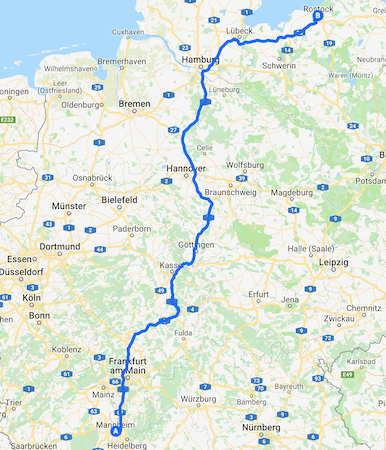
\includegraphics[scale=0.7]{route_1.png}} &
\subfloat[Route 2: Karlsruhe - Kandel]{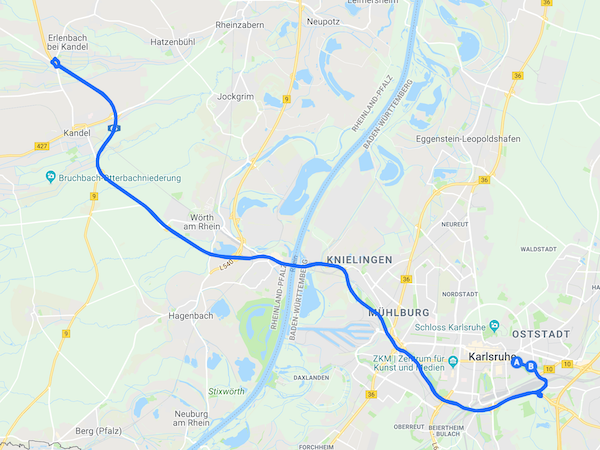
\includegraphics[scale=0.7]{route_2.png}} \\
\end{tabular}
\caption{Routen für die Aufnahme der realen Bilddaten \cite{google2018route1, google2018route2}}
\label{fig_strecken_real}
\end{figure}

Die Aufnahme der Route 1 umfasst über sechs Stunden Videomaterial mit über einer Stunde Fahrt auf einer 2-spurigen Autobahn \cite{youtube2018video}. Davon werden manuell zwischen 50 und 180 Szenarien aus jeder Klasse gelabelt. Da von den Szenarien \textit{lane change left} und \textit{lane change right} jeweils nur 50 Szenarien vorhanden sind, wird vom Autor eine Fahrt auf Route 2 mit einigen Spurwechseln aufgenommen. Das Ergebnis sind jeweils 17 weitere Szenarien in den Klassen \textit{lane change left} und \textit{lane change right}.Abbildung \ref{fig_beispiel_szenario_lcr_real} zeigt ein Beispiel des realen Szenarios \textit{lane change right} mit allen zugehörigen 15 Bildern.

\begin{figure}[h]
\centering
\begin{tabular}{c c c c c}
\subfloat[]{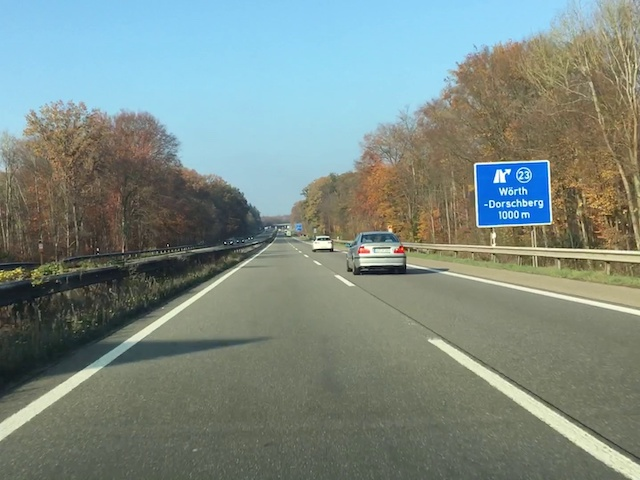
\includegraphics[scale=0.1]{lcr_real/frame0.jpg}} &
\subfloat[]{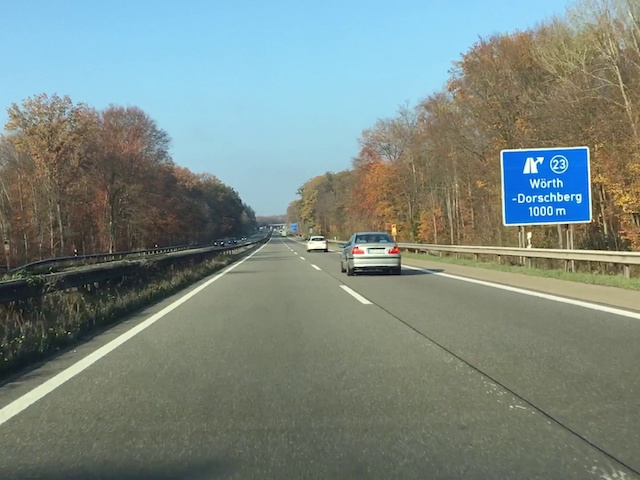
\includegraphics[scale=0.1]{lcr_real/frame1.jpg}} &
\subfloat[]{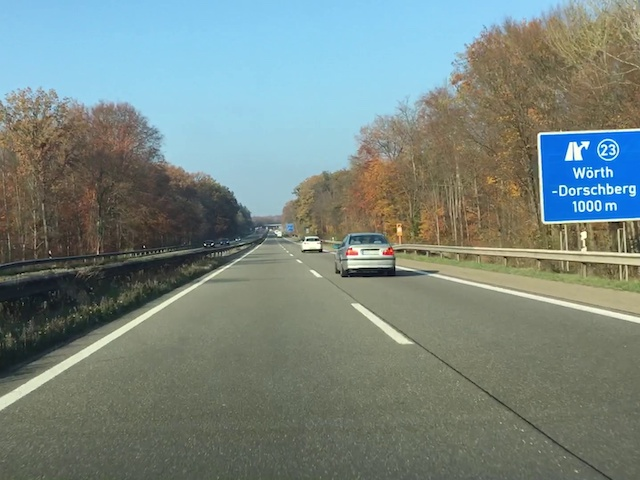
\includegraphics[scale=0.1]{lcr_real/frame2.jpg}} &
\subfloat[]{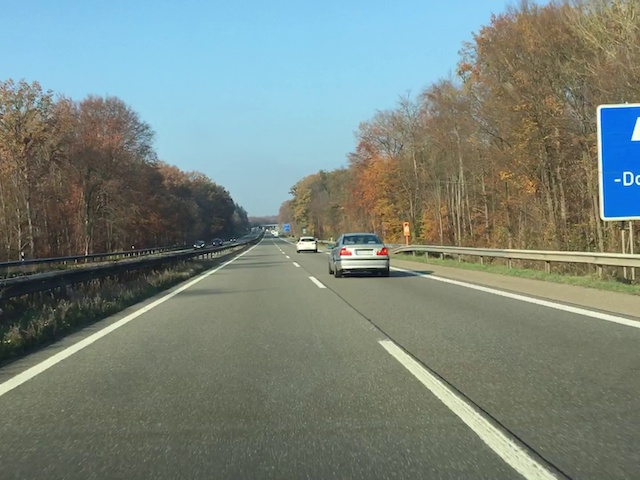
\includegraphics[scale=0.1]{lcr_real/frame3.jpg}} &
\subfloat[]{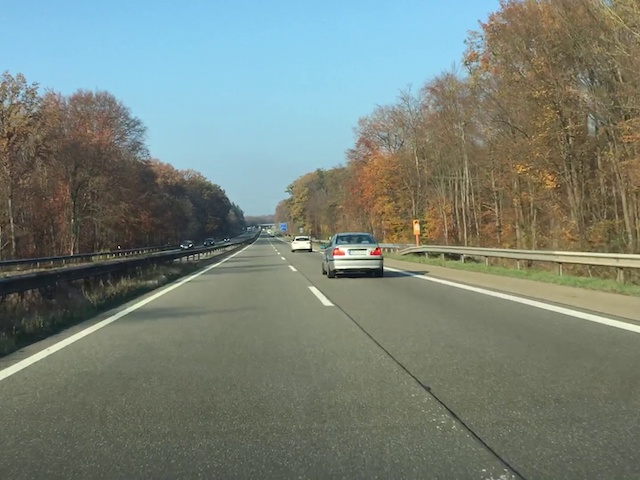
\includegraphics[scale=0.1]{lcr_real/frame4.jpg}} \\
\subfloat[]{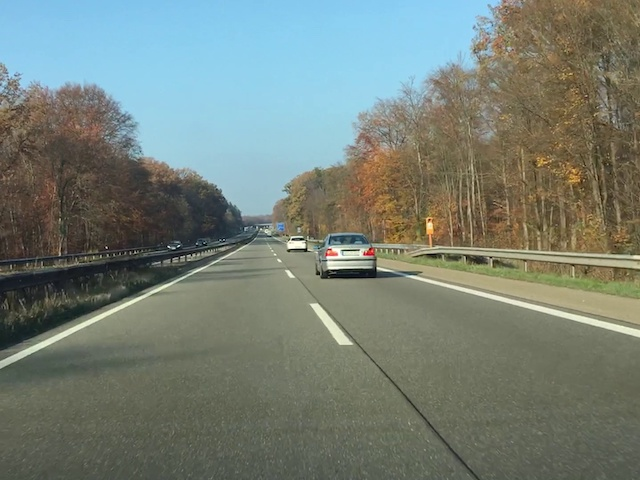
\includegraphics[scale=0.1]{lcr_real/frame5.jpg}} &
\subfloat[]{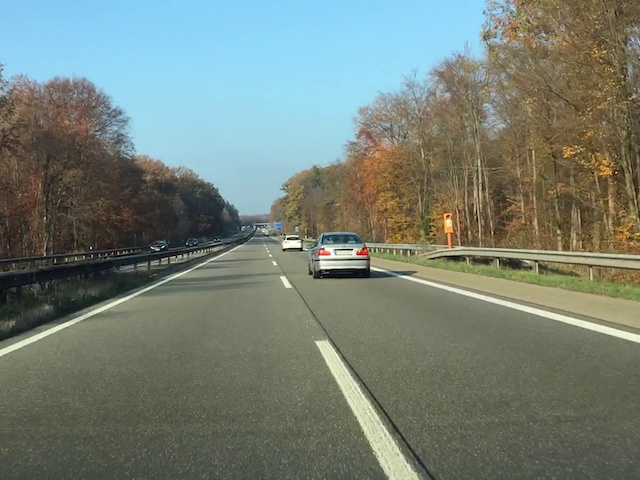
\includegraphics[scale=0.1]{lcr_real/frame6.jpg}} &
\subfloat[]{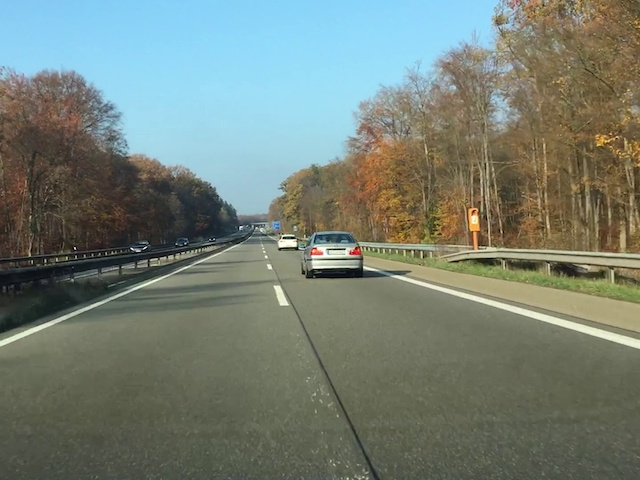
\includegraphics[scale=0.1]{lcr_real/frame7.jpg}} &
\subfloat[]{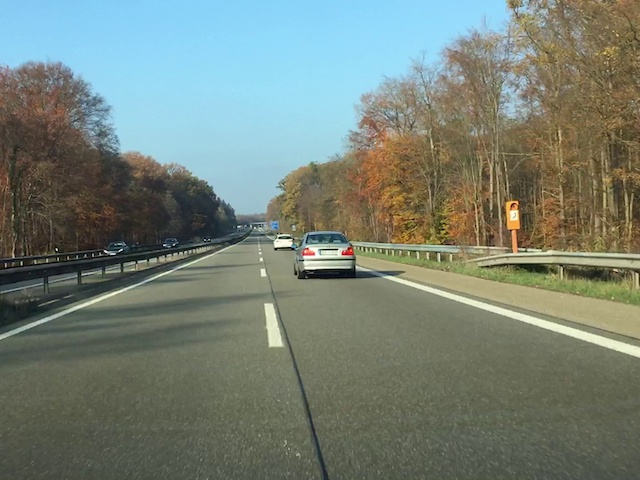
\includegraphics[scale=0.1]{lcr_real/frame8.jpg}} &
\subfloat[]{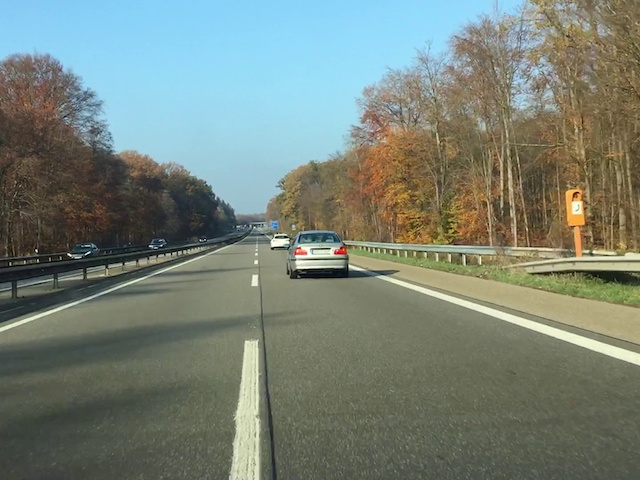
\includegraphics[scale=0.1]{lcr_real/frame9.jpg}} \\
\subfloat[]{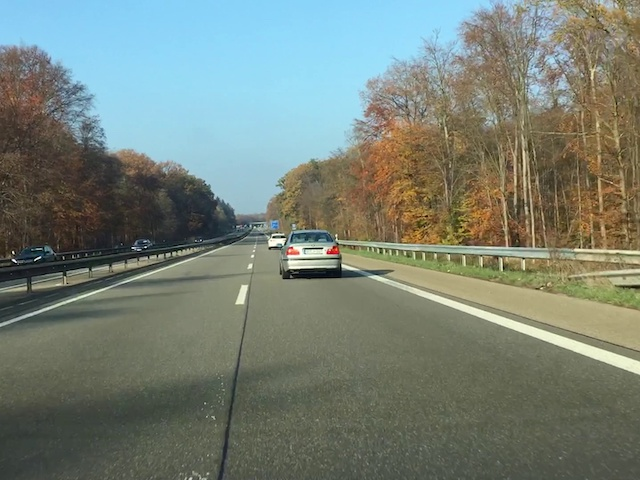
\includegraphics[scale=0.1]{lcr_real/frame10.jpg}} &
\subfloat[]{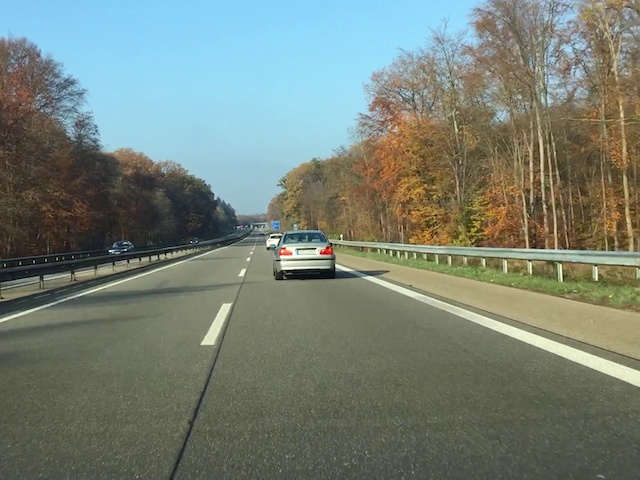
\includegraphics[scale=0.1]{lcr_real/frame11.jpg}} &
\subfloat[]{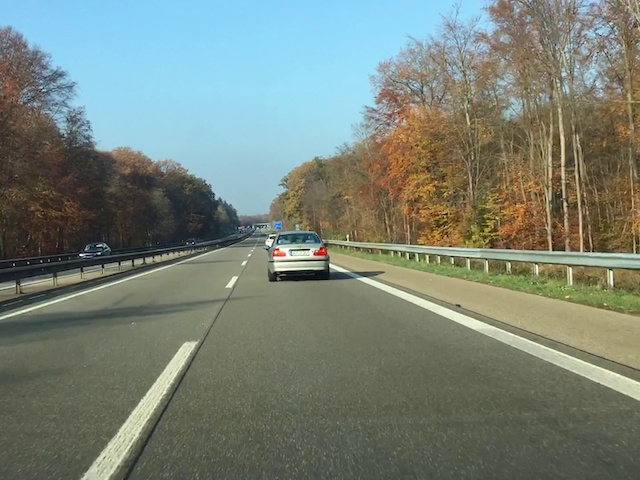
\includegraphics[scale=0.1]{lcr_real/frame12.jpg}} &
\subfloat[]{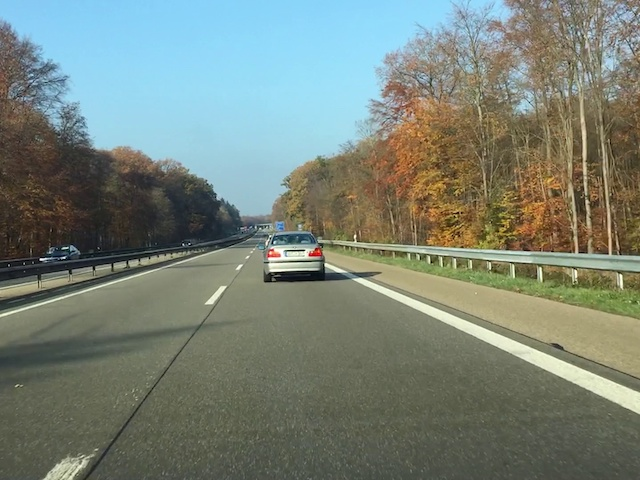
\includegraphics[scale=0.1]{lcr_real/frame13.jpg}} &
\subfloat[]{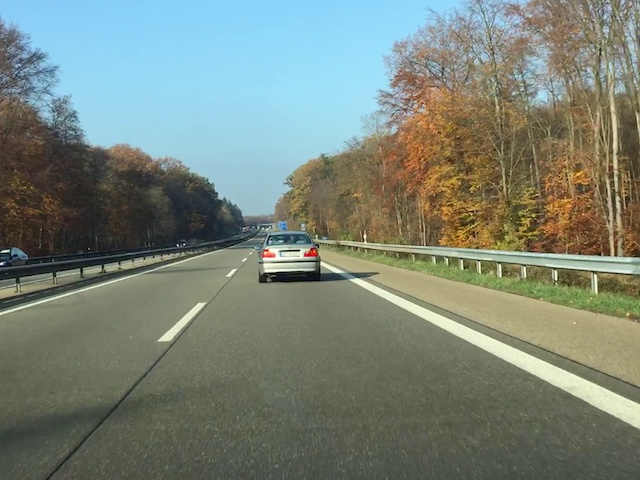
\includegraphics[scale=0.1]{lcr_real/frame14.jpg}} \\
\end{tabular}
\caption{Beispiel eines realen Szenarios der Klasse \textit{lane change right}}
\label{fig_beispiel_szenario_lcr_real}
\end{figure}


% ===========================
\section{Training}
\label{umsetzung_training}
% ===========================

In diesem Abschnitt wird zu Beginn das Format und der Import der Trainings- und Testdaten in das \ac{KNN} erklärt. Danach werden verschiedene Architekturen von \acp{KNN}, die in dieser Arbeit zum Einsatz kommen, vorgestellt und schließlich werden die durchgeführten Experimente mit diesen Architekturen erläutert. Die Vorbereitung der Daten und das Training wird mit Python und der Deep-Learning-Bibliothek Keras \cite{chollet2015keras} implementiert.


% ===========================
\subsection{Inputdaten}
\label{umsetzung_training_input}
% ===========================

Die Generierung der synthetischen und realen Trainings- und Testdaten wurde bereits in den vorherigen Abschnitten beschrieben. In diesem Abschnitt soll kurz darauf eingegangen werden wie diese Daten in das jeweilige \ac{KNN} eingespeist werden.

In dieser Arbeit werden \acp{CNN} für die Erkennung einzelner Bilder und Kombinationen aus \acp{CNN} und \ac{LSTM} für die Klassifizierung von Videos eingesetzt. Daher müssen sowohl einzelne Bilder, als auch Bildsequenzen in das jeweilige \ac{KNN} importiert werden. Da es sich um große Datenmengen von über 50GB handelt, müssen die Daten mit einem Datenstrom eingespeist werden, da nicht alle Daten zu Beginn in den Arbeitsspeicher geladen werden können.

Die Deep-Learning-Bibliothek Keras hat bereits sogenannte \textit{DataGenerators} für der Import von einzelnen Bildern und für sequenzielle Daten mit zwei Dimensionen (e.g. CSV-Dateien). Es gibt allerdings keine bereits nutzbare Lösung für den Import von sequentiellen Bildern, was 4-dimensionalen Daten entspricht (Anzahl Bilder, Höhe, Breite, Farbkanal). Aus diesem Grund wird die Lösung von Amidi \ref{amidi2017datagenerator} adaptiert um höher-dimensionale Datensets importieren zu können.

Von den generierten synthetischen und realen Szenarien werden \textit{free cruising}, \textit{following}, \textit{catching up}, \textit{lane change left} und \textit{lane change right} für das Training ausgewählt. Das Szenario \textit{approaching} wurde für den Proof-of-Concept in dieser Arbeit bewusst entfernt, weil es oft Überscheidungen mit dem Szenario \textit{following} gibt. Diese Überschneidungen und Ähnlichkeiten zwischen Szenarien und ihren Einfluss auf das Training eines Klassifikators können in weiteren Arbeiten untersucht werden. Das Szenario \textit{overtaking} wurde entfernt, weil es mit der konfigurierten Frontkamera allein nicht erfasst werden kann. In folgenden Arbeiten kann dieses Szenario mithilfe weiterer Kameraperspektiven zusätzlich berücksichtigt werden.

Um das Ergebnis nicht zu verzerren, sollten für das Training mit neuronalen Netzen in jeder Klasse jeweils die gleiche Anzahl an Trainings- und Testdaten vorhanden sein. Aus diesem Grund werden für das Training aus jeder Klasse nur die Anzahl der Szenarien verwendet, die mindestens in jeder Klasse verfügbar sind. Damit dieser Ansatz auch in der Praxis verwendet werden kann wird außerdem darauf geachtet, dass 95\% synthetische Daten und 5\% reale Daten für das Training verwendet werden. Mit dieser Verteilung bleibt der manuelle Aufwand für das Labeln der Trainingsdaten überschaubar. Die daraus resultierende Aufteilung von synthetischen und realen Szenarien auf Trainings-, Validierungs- und Testdaten ist in Tabelle \ref{tab_daten_aufteilung} aufgeschlüsselt. Beim Training mit einzelnen Bildern wird die gleiche Verteilung angewendet und da jedes Szenario aus 15 Bilder besteht, können die Zahlen aus Tabelle \ref{tab_daten_aufteilung} einfach mit 15 multipliziert werden.

\begin{table}[h]
\small
\centering
\def\arraystretch{1.4}
\begin{tabular}{l | c c c c c c | c}

& \multicolumn{3}{c}{\textbf{Synthetische Daten}} & \multicolumn{3}{c|}{\textbf{\textbf{Reale Daten}}} & \\
& Training & Validierung & Test & Training & Validierung & Test & \\
Szenario & 85\% & 10\% & 5\% & 65\% & 10\% & 25\% & Summe \\
\hline
free cruising & 807 & 95 & 48 & 43 & 7 & 17 & 1.017 \\
following & 807 & 95 & 48 & 43 & 7 & 17 & 1.017 \\
catching up & 807 & 95 & 48 & 43 & 7 & 17 & 1.017 \\
lane change left & 807 & 95 & 48 & 43 & 7 & 17 & 1.017 \\
lane change right & 807 & 95 & 48 & 43 & 7 & 17 & 1.017 \\
\hline
\textbf{Summe} & \textbf{4.035} & \textbf{475} & \textbf{240} & \textbf{215} & \textbf{35} & \textbf{85} & 5.085 \\
\hline

\end{tabular}
\caption{Aufteilung von synthetischen und realen Szenarios auf Trainings-, Validierungs- und Testdaten}
\label{tab_daten_aufteilung}
\end{table}

Die Bilddaten werden für das Training außerdem in die Form 299 x 299 x 3 Pixel transformiert. Diese Bildgröße ist ein Kompromiss zwischen Detailgrad und Trainingszeit und wird in Keras, neben der Auflösung 244 x 244 x 3 Pixel, für \acp{CNN} als Standardkonfiguration vorgeschlagen \cite{chollet2015keras}.

% ===========================
\subsection{Architektur der künstlichen neuronalen Netze}
\label{umsetzung_training_architektur}
% ===========================

In diesem Abschnitt werden verschiedene Architekturen von tiefen \acp{KNN} vorgestellt, die im nächsten Abschnitt \ref{umsetzung_training_experimente} für die Experimente in dieser Arbeit verwendet werden. Wie in Abschnitt \ref{grundlagen_nn_video} erläutert, gibt es verschiedenen Ansätze um Bildsequenzen mit \acp{KNN} zu klassifizieren. In dieser Arbeit werden zwei unterschiedliche Ansätze umgesetzt und miteinander verglichen. Im ersten Ansatz werden die Bilder in den Sequenzen einzeln klassifiziert. Anschließend wird den Sequenzen die Klasse zugeordnet, mit der die meisten Bilder in der Sequenz klassifiziert wurden. Für den zweiten Ansatz wird eine Kombination aus Bild- und Sequenzerkennung verwendet um die Bildsequenzen als ganzes zu klassifizieren. Die Architekturken für den jeweiligen Ansatz werden in den folgenden Absätzen vorgestellt.

Beim ersten Ansatz handelt es sich um die Klassifizierung von einzelnen Bildern, wofür \acp{CNN} verwendet werden. Das Training mit \acp{CNN} hat in den vergangenen Jahre große Fortschritte gemacht durch die Verfügbarkeit von großen Datenmengen, steigender Rechenleistung und die Wiederverwendung von bereits vortrainierten \acp{CNN}. Diese Verwendung von bereits trainierten Netzen nennt sich Transferlernen (engl. transfer learning) \cite{oquab2014transfer}. Die Idee von einem \ac{CNN} ist es in den frühen Schichten sehr grundlegende Merkmale (engl. low-level features) und in späteren Schichten abstraktere Merkmale (engl. high-level features) zu extrahieren. Schließlich wird Bilder auf Basis dieser abstrakten Merkmale mithilfe von einer oder mehreren Fully-Connected-Schichten klassifiziert. Diese Funktionsweise macht man sich beim Transferlernen zunutze und verwendet ein \ac{CNN} das bereits auf vielen Millionen Bildern trainiert wurde. Dieses \ac{CNN} hat bereits gelernt unterschiedliche Merkmale aus Bildern zu extrahieren. Um ein ein solches neuronales Netz für die eigene Arbeit verwenden zu können, muss man lediglich die letzten Fully-Connected-Schichten ersetzen und mit den eigenen Bilddaten und entsprechenden Klassen trainieren \cite{oquab2014transfer}. Mit diesem Verfahren kann viel Zeit und Rechenleistung gespart werden, weil die grundlegende Merkmalsextraktion nicht grundlegend neu gelernt werden muss. 

Das Transferlernen wird auch in dieser Arbeit verwendet. Dazu wurden verschiedene \ac{CNN}-Architekturen verglichen und schließlich zwei unterschiedliche für diese Arbeit ausgewählt. Eine Übersicht der bekanntesten vortrainierten \acp{CNN} ist in Abbildung \ref{fig_comparison_cnns} dargestellt. In dieser Darstellung werden die neuronalen Netze anhand ihrer erreichen Genauigkeit (engl. accuracy) und der benötigten Operationen bzw. ihrer Parameter bei der Berechnung einer Klassifizierung eingeordnet \cite{canziani2016analysis}.

\begin{figure}[h]
\centering
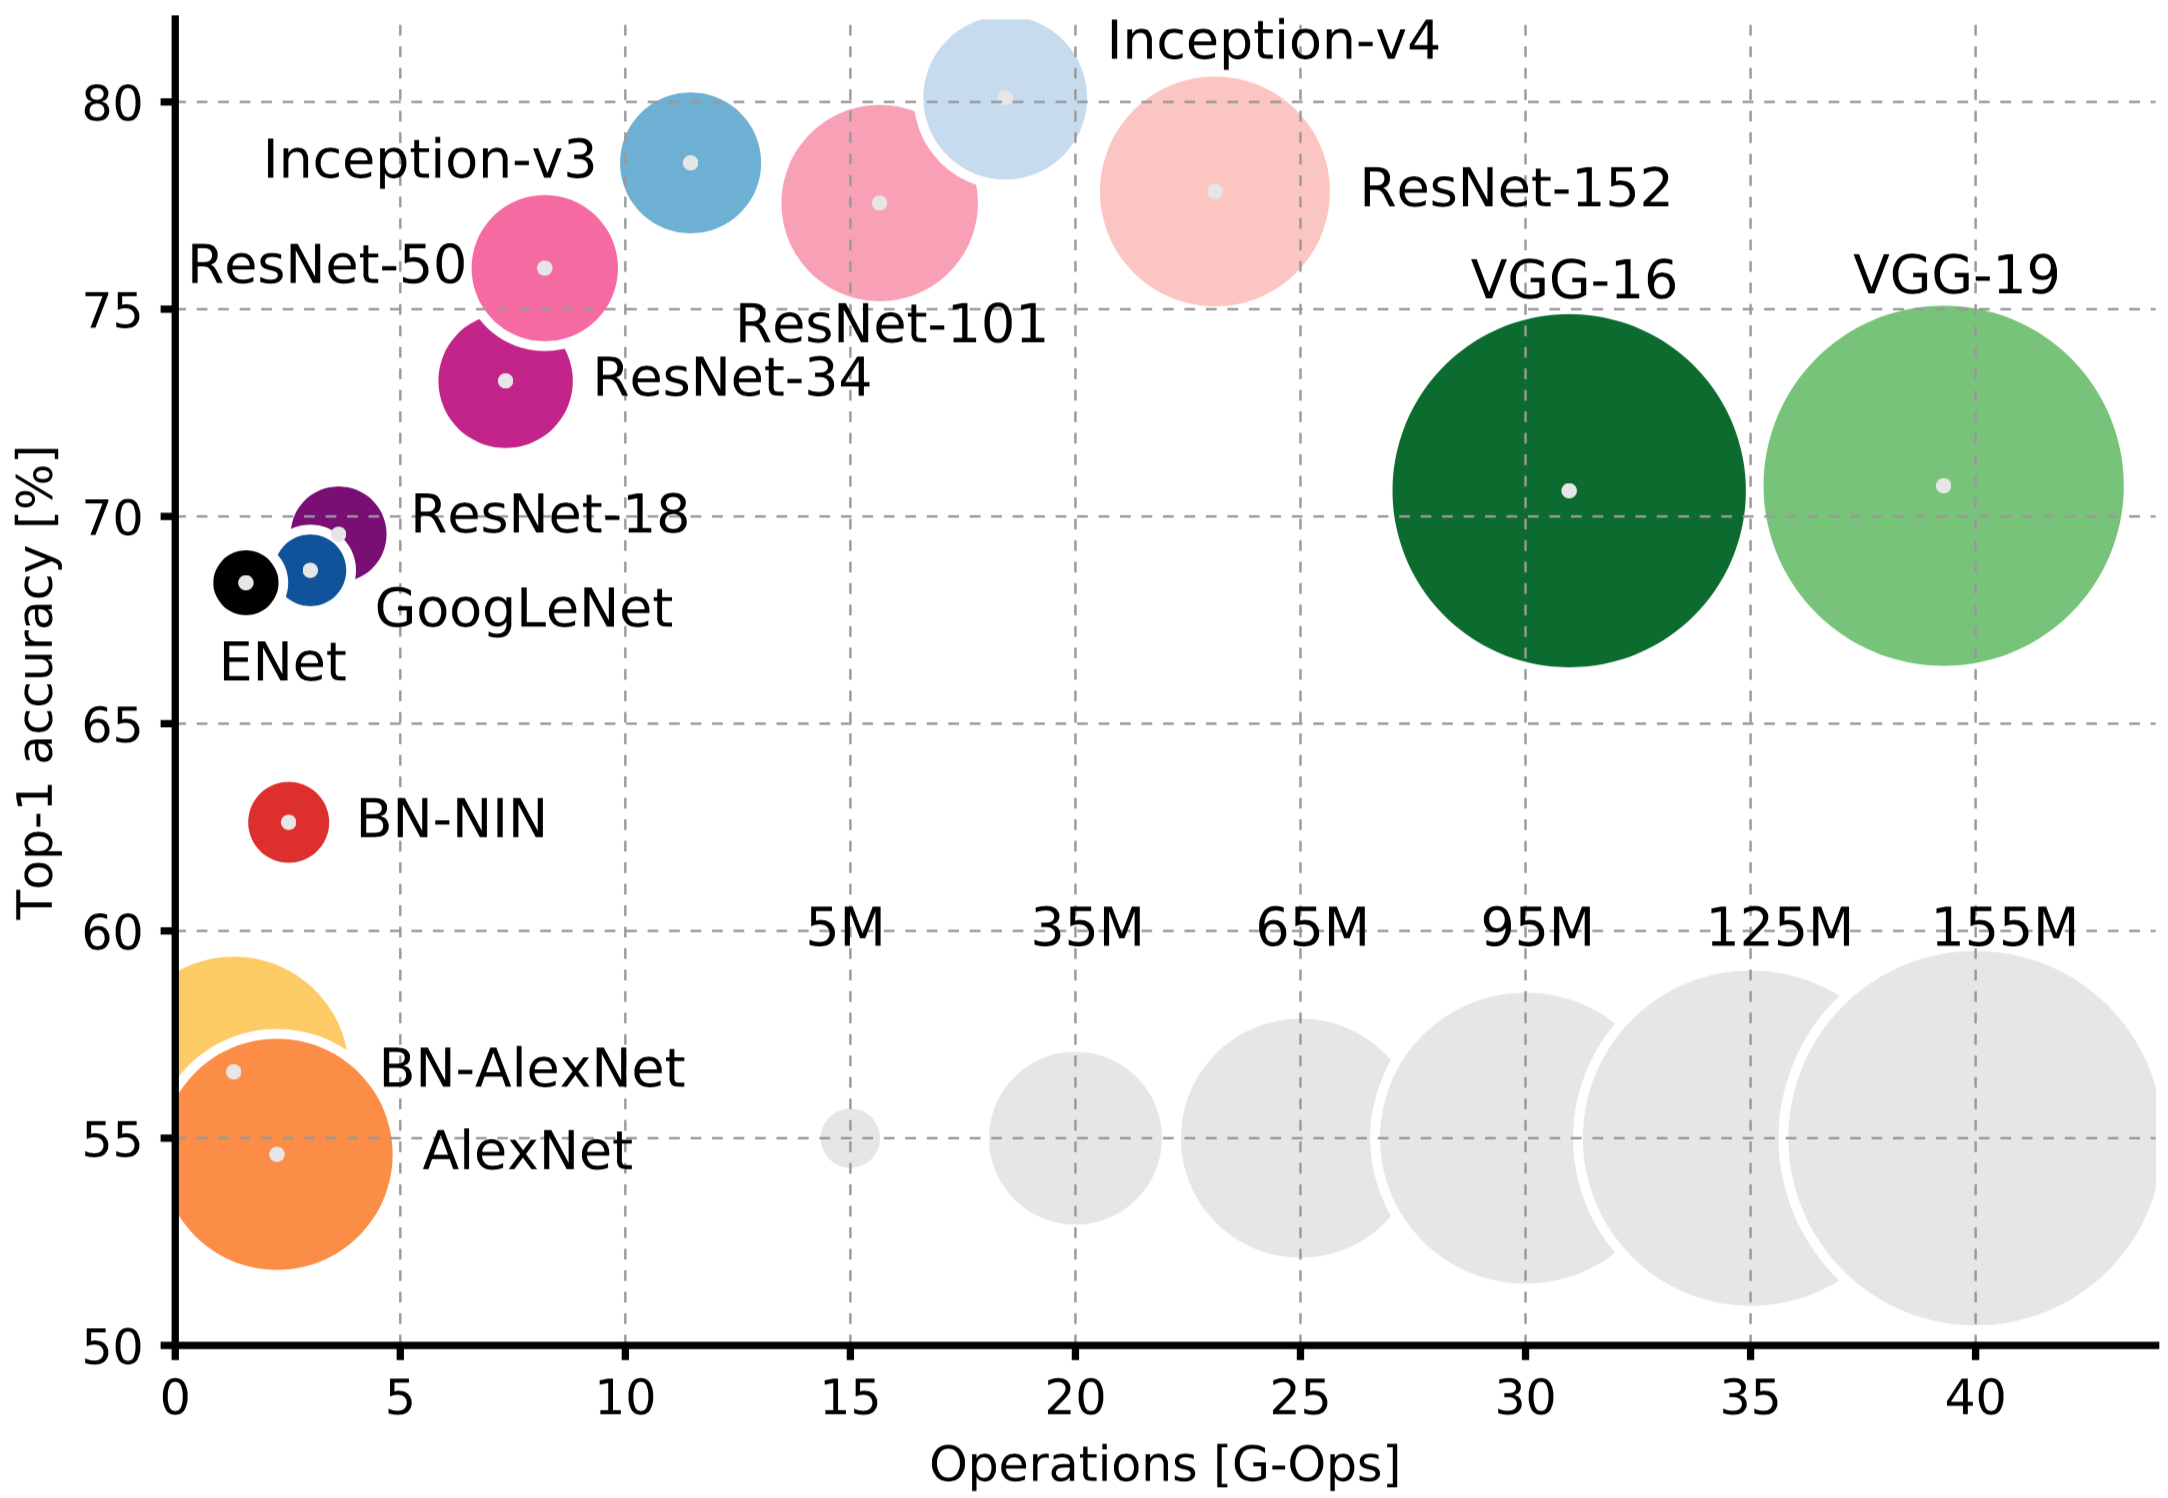
\includegraphics[scale=0.35]{comparison_cnns.png}
\caption{Vergleich von vortrainierten \aclp{CNN}, entnommen aus \cite{canziani2016analysis}}
\label{fig_comparison_cnns}
\end{figure}

Für die Architekturen in dieser Arbeit werden die \acp{CNN} Inception-V3 \cite{szegedy2016inception} und VGG-16 \cite{simonyan2014vgg} als Basis verwendet, weil beide in vergangene Wettbewerben und anderen Arbeiten sehr gute Ergebnisse erzielen konnten.

Das VGG-16 Netz 
138,357,544

ImageNet ist ein Datensatz mit 14.197.122 Bildern und 21.841 sogenannten Synonymmengen (engl. synonym sets) \cite{deng2009imagenet}. In Synonymmengen sind Wörter der gleichen Bedeutung zusammengefasst. Dabei sind alle Wörter auch hierarchisch nach dem WordNet-Projekt eingeordnet.

Im Gegensatz zu einfach gestapelten Convolution- und Pooling-Schichten wie beispielsweise dem VGG-16 Netz, orientiert sich das Inception-V3 Netz an zusätzlichen Prinzipen, um die Genauigkeit zu verbessern und die Rechenleistung zu senken. Zusätzlich werden Convolution-Operationen nicht nur gestapelt, sondern auch parallel zu anderen Convolution-Operationen berechnet, was zu einer besseren Leistung des Netzes führt \cite{szegedy2016inception}. 

Es wird argumentiert, dass ein Filter mit der Dimension 5x5 durch zwei aufeinanderfolgende Filter der Dimension 3x3 ersetzt werden kann, was die Rechenleistung deutlich reduziert \cite{szegedy2016inception}. Diese Funktionalität wird in einem sogenannten Inception-Modul umgesetzt, was in Abbildung \ref{fig_inc_fig} unter (a) zu sehen ist. Ein weiteres Prinzip ist, dass ein nxn-Filter mit einen 1xn-Filter gefolgt von einem nx1 Filter ersetzt werden kann, bei gleichbleibender Leistung und 33\% weniger Rechenaufwand. Dieses Prinzip ist in Abbildung \ref{fig_inc_fig} unter (b) dargestellt. Für das dritte Prinzip wird argumentiert, dass bei einer starken Dimensionsreduzierung durch Pooling-Schichten viel Information aus dem Bild verloren gehen kann. Um dies zu verhindern, werden statt einer Pooling-Schicht mehrere parallele Convolution-Operationen ausgeführt. Dieses Prinzip wird mit dem Inception-Modul aus Abbildung \ref{fig_inc_fig} unter (c) umgesetzt.

\begin{figure}[h]
\centering
\begin{tabular}{c c}
\subfloat[Inception-Modul in dem ein 5x5-Filter mit zwei 3x3-Filter ersetzt wird]{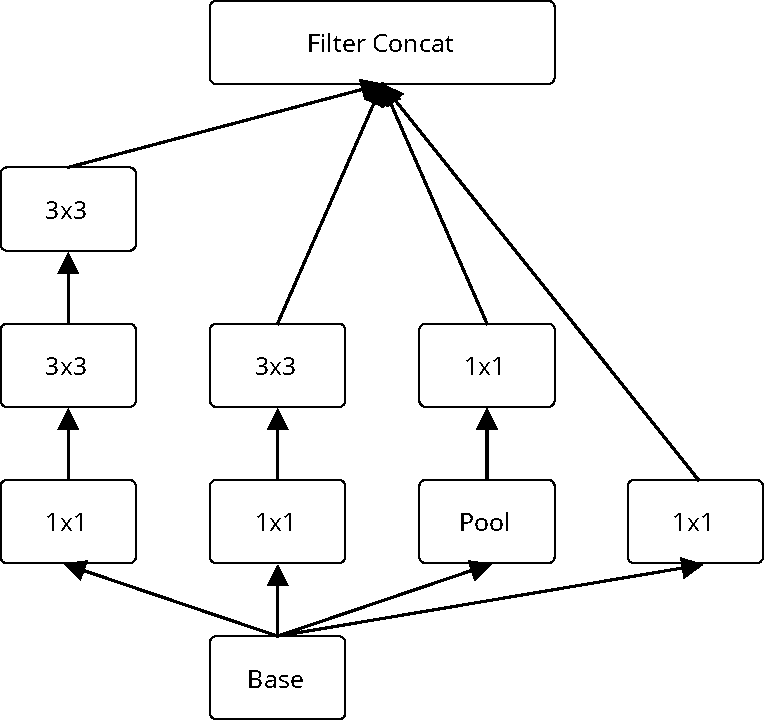
\includegraphics[scale=0.35]{inc_fig_5.pdf}} &
\subfloat[Inception-Modul in dem ein 7x7-Filter mit einen 1x7-Filter gefolgt von einem 7x1 Filter ersetzt wird]{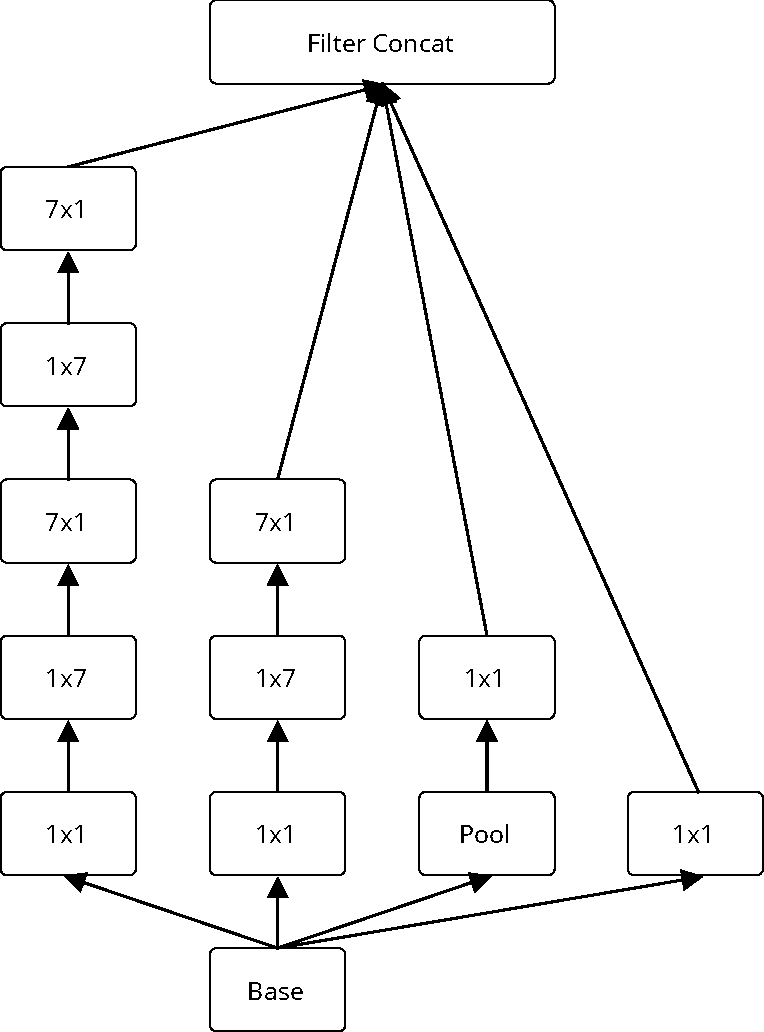
\includegraphics[scale=0.35]{inc_fig_6.pdf}} \\
\subfloat[Inception-Modul in statt einer Pooling-Schicht mehrere parallele Convolution-Operationen ausgeführt werden]{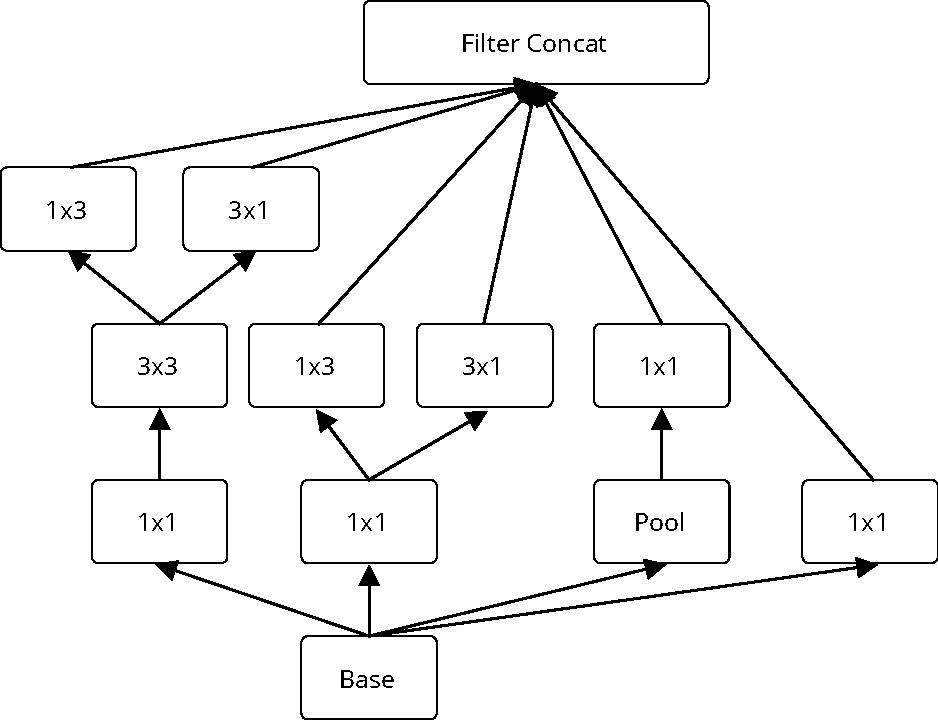
\includegraphics[scale=0.35]{inc_fig_7.pdf}} &
\end{tabular}
\caption{Inception-Module aus der Inception-V3 Architektur \cite{szegedy2016inception}}
\label{fig_inc_fig}
\end{figure}

Die Architektur des gesamten Netzes ist in Abbildung \ref{fig_inception_v3} dargestellt. In dieser Arbeit wird ein Inception-V3 Netz verwendet, das mit dem Datenset ImageNet \cite{deng2009imagenet} trainiert wurde.

\begin{figure}[h]
\centering
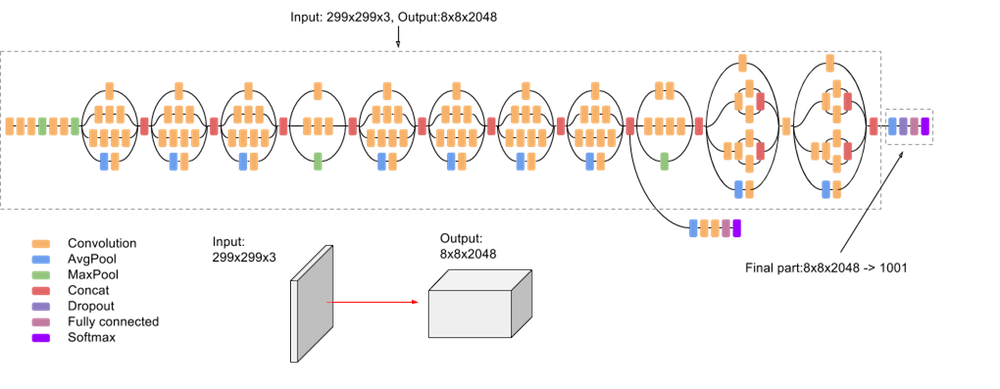
\includegraphics[scale=0.45]{inception_v3.png}
\caption{Architektur des Inception-V3 Netzes, entnommen aus \cite{google2018inceptionv3}}
\label{fig_inception_v3}
\end{figure}



% ===========================
\subsection{Experimente}
\label{umsetzung_training_experimente}
% ===========================

 Stet clita kasd gubergren, no sea takimata sanctus est Lorem ipsum dolor sit amet. Lorem ipsum dolor sit amet, consetetur sadipscing elitr, At accusam aliquyam diam diam dolore dolores duo eirmod eos erat, et nonumy sed tempor et et invidunt justo labore Stet clita ea et gubergren, kasd magna no rebum. sanctus sea sed takimata ut vero voluptua. est Lorem ipsum dolor sit amet. Lorem ipsum dolor sit amet, consetetur
 
 Dropout - \cite{hinton2012improving}
 \cite{srivastava2014dropout}

 
 

